\documentclass[12pt,aspectratio=169,handout]{beamer}
\usepackage[T1]{fontenc}
\usepackage{lmodern}
\usepackage{amsmath,amssymb,array,booktabs,tabularx,tikz}
% Add language support appropriate to the source, if needed.
% Keep this preamble inline in every delivered deck.
\definecolor{GEInk}{HTML}{132A3E}
\definecolor{GETeal}{HTML}{17675E}
\definecolor{GEFooter}{HTML}{EAF2F1}
\setbeamercolor{background canvas}{bg=white}
\setbeamercolor{normal text}{fg=GEInk,bg=white}
\setbeamercolor{structure}{fg=GETeal}
\setbeamercolor{frametitle}{fg=GEInk}
\setbeamercolor{GE footer}{fg=GETeal,bg=GEFooter}
\setbeamerfont{normal text}{family=\sffamily,size=\normalsize}
\setbeamerfont{title}{size=\huge,series=\bfseries}
\setbeamerfont{subtitle}{size=\normalsize,series=\bfseries}
\setbeamerfont{frametitle}{size=\Large,series=\bfseries}
\setbeamerfont{framesubtitle}{size=\normalsize,series=\mdseries}
\setbeamerfont{GE footer}{size=\footnotesize}
\setbeamersize{text margin left=9mm,text margin right=9mm}
\setbeamertemplate{navigation symbols}{}
\setbeamertemplate{headline}{}
\setbeamercovered{invisible}

% Structural hierarchy adapted from Worked Example 1; independent of highlights.
\newcommand{\TaskName}[1]{\ifcase#1\or
Establish the binary model and monetary transformations.\or
Individual expected values.\fi}
\newcommand{\SubtaskName}[2]{\ifcase#1\or
  \ifcase#2\or Binary model and monetary transformations.\or
  Supports, PMFs, and ordered CDFs.\or Initial probabilities and loss events.\fi
\or
  \ifcase#2\or Initial expected values.\or
  Expectation formulas and sign intervals.\or Graphs.\fi
\fi}
\newcommand{\TaskHeading}[1]{%
  \par\noindent\tikz[baseline=(tasktitle.base)]{%
    \node[fill=black!5,text=GEInk,rounded corners=2mm,
      inner xsep=4pt,inner ysep=3pt,outer sep=0pt,
      text width=\dimexpr\linewidth-8pt\relax,align=left,
      font=\footnotesize\bfseries] (tasktitle) {Task #1 --- \TaskName{#1}};}\par}
\newcommand{\SubtaskHeading}[2]{%
  \par\noindent
  {\normalsize\bfseries\underline{#2. \SubtaskName{#1}{#2}}\par}}
\newcommand{\ActiveTask}{0}
\newcommand{\ActiveSubtask}{0}
\newcommand{\SetTaskSubtask}[2]{\renewcommand{\ActiveTask}{#1}%
  \renewcommand{\ActiveSubtask}{#2}}
\newcommand{\TaskBody}{\setlength{\parskip}{0pt}}
\newcommand{\ActiveHierarchy}{%
  \begingroup\setlength{\parskip}{0pt}
  \ifnum\ActiveTask>0
    \TaskHeading{\ActiveTask}\vskip2pt
    \SubtaskHeading{\ActiveTask}{\ActiveSubtask}\vskip3pt
  \fi\endgroup}

\setbeamertemplate{frametitle}{%
  \raggedright\setlength{\parskip}{0pt}
  \vskip.3em
  \ActiveHierarchy
  {\usebeamerfont{frametitle}\strut\insertframetitle\strut\par}%
  \ifx\insertframesubtitle\empty\else
    {\usebeamerfont{framesubtitle}\strut\insertframesubtitle\strut\par}%
  \fi
  \vskip.25em
}
\setbeamertemplate{footline}{%
  \begin{beamercolorbox}[wd=\paperwidth,ht=3ex,dp=1.3ex,
    leftskip=9mm,rightskip=9mm]{GE footer}%
    \usebeamerfont{GE footer}\insertsectionhead\hfill
    \insertframenumber/\inserttotalframenumber
  \end{beamercolorbox}%
}
\setlength{\parindent}{0pt}
\setlength{\parskip}{.35em}
\setlength{\tabcolsep}{4pt}
\renewcommand{\arraystretch}{1.22}
\AtBeginEnvironment{frame}{\raggedright}
\addtobeamertemplate{frametitle}{}{%
  \setlength{\abovedisplayskip}{6pt plus 2pt minus 2pt}%
  \setlength{\belowdisplayskip}{6pt plus 2pt minus 2pt}%
  \setlength{\abovedisplayshortskip}{6pt plus 2pt minus 2pt}%
  \setlength{\belowdisplayshortskip}{6pt plus 2pt minus 2pt}%
}


% Resolved coordinated palette: highlights_palette.tex, base and registry palettes.
\definecolor{GTenHLValue}{HTML}{FFBB55}
\definecolor{GTenHLSecond}{HTML}{8FD49A}
\definecolor{GTenHLOutcome}{HTML}{BC9DE0}
\definecolor{GTenHLProbability}{HTML}{86BFF0}
\definecolor{CriticalColor}{HTML}{2648BB}
\colorlet{G10T2C3FunctionColor}{GTenHLSecond!85!black}
\colorlet{MathHLSuccessColor}{GTenHLProbability!65!CriticalColor}
\definecolor{MathHLComplementColor}{HTML}{D74383}
\definecolor{MathHLCumulativeColor}{HTML}{43A5C9}
\definecolor{ExpectedValueColor}{HTML}{D6A52A}

% Use \definecolor{MeaningfulRoleName}{HTML}{...} for each used role.
% Slide-only padding per side, shared by every semantic highlight wrapper.
\newlength{\GEHighlightVerticalPadding}
\setlength{\GEHighlightVerticalPadding}{.5mm}
\tikzset{ge marker/.style={rectangle,rounded corners=1mm,draw=none,
  fill=#1,fill opacity=.32,text opacity=1,text=GEInk,
  inner xsep=.6mm,inner ysep=\GEHighlightVerticalPadding,outer sep=0pt}}
\newif\ifGTenHighlights
\GTenHighlightsfalse
% \GTenHighlightsfalse % Uncomment to disable instructional highlights.
% Preserve an existing source toggle setting when adapting a deck.
\makeatletter
\newcommand{\GEHighlightMath}[2]{%
  \tikz[baseline=(gehl.base)]\node[ge marker=\GECurrentRole]
    (gehl) {$\m@th#1#2$};}
\newcommand{\GEHighlight}[2]{%
  \ifGTenHighlights
  \begingroup\def\GECurrentRole{#1}%
  \ifmmode\mathpalette\GEHighlightMath{#2}%
  \else\tikz[baseline=(gehl.base)]\node[ge marker=#1](gehl){#2};\fi
  \endgroup
  \else#2\fi}
\makeatother
% Keep rows, rules, and table structure outside this space-reserving command.
\newcommand{\GERevealCell}[2]{\leavevmode\visible<#1->{#2}}


% All aliases share the single slide-only padding parameter and disabled branch.
\newcommand{\GTenHLValue}[1]{\GEHighlight{GTenHLValue}{#1}}
\newcommand{\GTenHLSecond}[1]{\GEHighlight{GTenHLSecond}{#1}}
\newcommand{\HLMathEvent}[1]{\GEHighlight{GTenHLOutcome}{#1}}
\newcommand{\HLProbability}[1]{\GEHighlight{GTenHLProbability}{#1}}
\newcommand{\HLSuccessProbability}[1]{\GEHighlight{MathHLSuccessColor}{#1}}
\newcommand{\HLComplementProbability}[1]{\GEHighlight{MathHLComplementColor}{#1}}
\newcommand{\HLCumulativeProbability}[1]{\GEHighlight{MathHLCumulativeColor}{#1}}
\newcommand{\HLExpectedValue}[1]{\GEHighlight{ExpectedValueColor}{#1}}
\newcommand{\HLGtenCThreeFunction}[1]{\GEHighlight{G10T2C3FunctionColor}{#1}}
\newcommand{\HLMathContext}[1]{#1}
\let\I\GTenHLValue
\let\M\GTenHLSecond
\let\A\HLMathEvent
\let\S\HLSuccessProbability
\let\Q\HLComplementProbability
\let\V\HLExpectedValue
\let\T\HLGtenCThreeFunction
\let\Prob\HLProbability
\let\CDF\HLCumulativeProbability
\newcommand{\EV}[1]{\V{\mathbb E}[\M{Y_{#1}}]}
\newcommand{\Ask}[1]{\textbf{#1}\par\smallskip}
\newcommand{\LegendTable}[1]{\begingroup\small
\begin{tabularx}{\linewidth}{@{}>{\raggedright\arraybackslash}p{.34\linewidth}>{\raggedright\arraybackslash}p{.25\linewidth}>{\raggedright\arraybackslash}X@{}}
\toprule\textbf{Symbol or notation}&\textbf{Concept}&\textbf{Brief meaning}\\\midrule
#1\bottomrule\end{tabularx}\par\endgroup}
\ifGTenHighlights
\colorlet{ExpectedInk}{ExpectedValueColor!55!black}
\colorlet{ProbabilityInk}{MathHLSuccessColor!50!black}
\else\colorlet{ExpectedInk}{black}\colorlet{ProbabilityInk}{black}\fi
\newcommand{\LegendOne}{\LegendTable{%
$\HLMathEvent{E}$, $\HLMathEvent{E^c}$ & \HLMathEvent{Event} \HLMathEvent{and} \HLMathEvent{complement} & Outcomes meeting a condition; those outside it.\\[5pt]
$\GTenHLValue{X}$, $\GTenHLValue{x}$ & \GTenHLValue{Primary} \GTenHLValue{variable} \GTenHLValue{and} \GTenHLValue{value} & Numerical rule and possible value; state the units.\\[5pt]
$\GTenHLValue{S_X}=\{\GTenHLValue{x}:\HLProbability{P}(\GTenHLValue{X}=\GTenHLValue{x})>0\}$ & \GTenHLValue{Support} & Distinct values with positive probability, in the variable's units.\\[5pt]
$\HLSuccessProbability{p}=\HLSuccessProbability{P}(\GTenHLValue{X}=\GTenHLValue{1})$ & \HLSuccessProbability{Success} \HLSuccessProbability{probability} & Chance of the specified state labelled 1, between 0 and 1.\\[5pt]
}}
\newcommand{\LegendTwo}{\LegendTable{%
$\HLComplementProbability{1-p}$ & \HLComplementProbability{Complement} \HLComplementProbability{probability} & Chance of the complementary state labelled 0.\\[5pt]
$\GTenHLSecond{Y_i}=f_i(\GTenHLValue{X})$ & \GTenHLSecond{Second} \GTenHLSecond{or} \GTenHLSecond{transformed} \GTenHLSecond{variable} & Another numerical description, with its own units.\\[5pt]
$\HLGtenCThreeFunction{f},\HLGtenCThreeFunction{f_i}$ & \HLGtenCThreeFunction{Transformation} \HLGtenCThreeFunction{function} & \HLGtenCThreeFunction{Maps} \HLGtenCThreeFunction{indicator} \HLGtenCThreeFunction{states} \HLGtenCThreeFunction{to} \HLGtenCThreeFunction{monetary} \HLGtenCThreeFunction{outcomes.}\\[5pt]
$\HLProbability{m_X(x)}$, $\HLProbability{m_{Y_i}(y)}$ & \HLProbability{Probability} \HLProbability{and} \HLProbability{mass} & Unitless chance of an event or one supported value.\\[5pt]
}}
\newcommand{\LegendThree}{\LegendTable{%
$\HLCumulativeProbability{F_X(t)}$, $\HLCumulativeProbability{F_{Y_i}(t)}$ & \HLCumulativeProbability{Cumulative} \HLCumulativeProbability{probability} & Chance up to a cutoff; the left limit excludes the cutoff.\\[5pt]
$\HLExpectedValue{\mathbb E}[\GTenHLSecond{Y_i}]$ & \HLExpectedValue{Expected} \HLExpectedValue{value} & Probability-weighted average, in original units.\\[5pt]
$\HLSuccessProbability{p_i^*}$ & \HLSuccessProbability{Individual} \HLSuccessProbability{break-even} \HLSuccessProbability{probability} & Probability at which the specified expected net payoff is zero.\\[5pt]
$f_i(0),f_i(1)$ & \HLMathContext{Transformation} \HLMathContext{inputs} & Scale, fixed addition or state payoffs, with required units.\\[5pt]
}}

\title{Bernoulli Models and\\Individual Break-Even Analysis}
\subtitle{Grade 10 \textbar{} Term 2 \textbar{} Lesson 1 \textbar{} C3}
\author{}\date{}
\newcommand{\GEOfficialCriterion}{\textbf{C3:} Models binary economic outcomes with Bernoulli random variables, interpreting success and failure in contexts such as default, gain, loss, or claim occurrence.}
\setbeamertemplate{title page}{\raggedright\vfill
{\color{GETeal}\usebeamerfont{subtitle}\insertsubtitle\par}\medskip
{\color{GEInk}\usebeamerfont{title}\inserttitle\par}\bigskip
{\normalsize\GEOfficialCriterion\par}\vfill}
% SOURCE MAP (historical line numbers; identify current source by headings):
% Practice: book2026-2027/grade10/term_2/1-practice_activities/G10_T2_L1_C3_practice_activity.tex
% Classroom: book2026-2027/grade10/term_2/2-class_activities/G10_T2_L1_C3_classroom_activity.tex
% Selected ONLY worked example 1, Campus concert food stand or indoor games,
% classroom lines 220--435; Task 1 231--346, Task 2 349--432.
% Prerequisites: classroom 157--193, general tasks 198--213;
% practice Binary models and distributions 187--207 and notation reference.
% Metadata/criterion: classroom 153--158; source toggle enabled in practice.
% Registry: highlights_g10_t2.tex reference G10-T2-C3-coordinated, 2777--2781.
% Renderer: highlights_compat_ttwo.tex 525--550, defaults + notation overrides;
% inherited fields resolved above from highlights_g10_t2 and highlights_g11_t1.
% Palette aliases: highlights_palette.tex 55--74, 145--168; roles in highlights_roles.tex.
% SOURCE DISCREPANCY: 12 registered rows, but CoordinatedLegendRow suppresses
% role=context (highlights_tables.tex 169--180), so the live legend prints 11.
% User explicitly requests all 12. Include final Transformation inputs unchanged,
% uncolored, using the renderer's criterion notation override f_i(0),f_i(1).
% The other 11 rows reproduce the live renderer, including default inherited names.
% Opening and closing invoke the exact same three row macros. No context filtering.
% Transformation function name/brief are short baseline-aligned marker fragments
% split only at spaces for readable wrapping; text and color are unchanged.
% Hierarchy map: Task 1.1 observation/indicator/transformation and checks;
% Task 1.2 support/PMF/CDF prerequisites, distributions and endpoint supports;
% Task 1.3 initial probabilities and loss events. Task 2.1 expectation prerequisite
% and initial expectations; Task 2.2 varying-p formulas, roots and sign intervals;
% Task 2.3 graphs, endpoint/root checks and contextual interpretation.
% Frame comments below retain original frame identifiers for source traceability;
% Overview and sign-work continuations preserve the step-by-step reveals.
\begin{document}
\section{Bernoulli models}
\begin{frame}\titlepage\end{frame}
% Frame 2: live coordinated legend; resolved rows 1--4
\begin{frame}[t]{Highlight legend (1/3)}
\LegendOne
\end{frame}
% Frame 3: live coordinated legend; resolved rows 5--8
\begin{frame}[t]{Highlight legend (2/3)}
\LegendTwo
\end{frame}
% Frame 4: live coordinated legend; resolved rows 9--12
\begin{frame}[t]{Highlight legend (3/3)}
\LegendThree
\end{frame}
% Frame 5: classroom 221--229: full context and assumptions
\begin{frame}[t]{Worked example 1: the weekend choice}
\framesubtitle{Campus concert food stand or indoor games}

A student club compares two hypothetical fundraising choices for one weekend:
a \M{food stand} at a campus outdoor concert or an \M{indoor games afternoon}.

The concert either goes ahead or is cancelled. Initially it goes ahead on
\S{three out of every eight weekends}.
\medskip
Only one option would be chosen. Both depend on the \A{same concert outcome}.
All monetary amounts are net gains or losses in USD after food, room,
equipment and publicity costs, as applicable.

\end{frame}
% Frame 6: classroom 221--229: given data, not calculated answers
\begin{frame}[t]{The two alternatives: state payoffs}

\Ask{What does each alternative earn in each concert state?}
\begin{tabularx}{\linewidth}{@{}>{\raggedright\arraybackslash}Xrr@{}}
\toprule Concert state & Food stand & Indoor games\\\midrule
Goes ahead & \M{USD 105} & \M{USD $-30$}\\[5pt]
Cancelled & \M{USD $-45$} & \M{USD 90}\\\bottomrule
\end{tabularx}
\medskip
\visible<2->{The concert draws potential players away from games. If it is cancelled,
students seek an indoor alternative.}\par

\visible<3->{Each alternative has one strictly positive and one strictly negative payoff.}\par


\end{frame}
% Frame 7: classroom general tasks 198--213 and worked Tasks 1 and 2
\begin{frame}[t]{The questions we will answer (1/2)}
\TaskHeading{1}
\medskip
\SubtaskHeading{1}{1}
Define one observation, the two states, the indicator and both monetary rules.
\medskip
\SubtaskHeading{1}{2}
Give supports, complete PMFs and numerically ordered piecewise CDFs.
\medskip
\SubtaskHeading{1}{3}
Identify each loss event, its probability and its contextual meaning.
\end{frame}
\begin{frame}[t]{The questions we will answer (2/2)}
\TaskHeading{2}
\medskip
\SubtaskHeading{2}{1}
Calculate initial expectations and interpret them per weekend.
\medskip
\SubtaskHeading{2}{2}
Keep payoffs fixed; vary $p\in[0,1]$. Find each expectation formula,
its own break-even threshold and sign intervals.
\medskip
\SubtaskHeading{2}{3}
Draw separate labelled graphs and check endpoints and roots.
\end{frame}
% Frame 8: classroom worked example 1, Task 1 (231--346)
\SetTaskSubtask{1}{1}
\begin{frame}[t]{One observation, two exhaustive states}
\TaskBody

\Ask{What is one observation, and which event will be labelled success?}
\visible<2->{One observation is the club's net outcome over \textbf{one weekend}
for the chosen option.}\par

\medskip
\visible<3->{$\A{E}$: the concert goes ahead.\qquad
$\A{E^c}$: the concert is cancelled.}\par

\medskip
\visible<4->{These states are mutually exclusive (not both) and exhaustive
(one must occur). The event label \textbf{success} means $\A{E}$ occurs;
it need not mean a monetary profit.}\par


\end{frame}
% Frame 9: classroom worked example 1, Task 1 (231--346)
\SetTaskSubtask{1}{1}
\begin{frame}[t]{Encode the event with a Bernoulli indicator}
\TaskBody

\Ask{How do we encode the two states numerically?}
\visible<2->{\[\I{X}=\begin{cases}\I{1}&\text{on }\A{E},\\\I{0}&\text{on }\A{E^c}.\end{cases}\]
The indicator $\I{X}$ is unitless.}\par

\visible<3->{\[\S{p}=P(\A{E})=P(\I{X}=\I{1})=\S{\frac38},\qquad
\Q{1-p}=P(\A{E^c})=\Q{1-\frac38}=\Q{\frac58}.\]}\par

\visible<4->{$\I{X}\sim\operatorname{Bernoulli}(\S{p}),\qquad
\S{p}+\Q{1-p}=1.$
}\par


\end{frame}
% Frame 10: classroom prerequisites 157--193 and worked transformation formulas 238--262
\SetTaskSubtask{1}{1}
\begin{frame}[t]{From a state to money: the general rule}
\TaskBody

\Ask{How can one formula reproduce both state payoffs?}
\visible<2->{$\T{f_i}:\{0,1\}\to\mathbb R$ maps an indicator state to money.
$\M{Y_i}=\T{f_i}(\I{X})$ is net profit in USD; $i$ identifies the alternative.}\par

\visible<3->{\[\M{Y_i}=\M{f_i(0)}+[\M{f_i(1)}-\M{f_i(0)}]\I{X}.\]}\par

\visible<4->{At $\I{X}=\I{0}$ the added term vanishes: the result is $\M{f_i(0)}$.
At $\I{X}=\I{1}$ the change is added: the result is $\M{f_i(1)}$.}\par

\medskip
\visible<5->{Both monetary variables use this same $\I{X}$; only one alternative is chosen.}\par


\end{frame}
% Frame 11: classroom worked example 1, Task 1 (231--346)
\SetTaskSubtask{1}{1}
\begin{frame}[t]{Derive the food stand transformation}
\TaskBody

\Ask{What is $Y_1$ as a constant plus a coefficient times $X$?}
$\M{f_1(0)}=\M{-45}$; $\M{f_1(1)}=\M{105}$ USD.
\[\begin{aligned}
\visible<2->{\M{Y_1}}&\visible<2->{=\M{f_1(0)}+[\M{f_1(1)}-\M{f_1(0)}]\I{X}}\\[5pt]
&\visible<3->{=\M{-45}+[\M{105}-(\M{-45})]\I{X}}\\[5pt]
&\visible<4->{=\M{-45}+\M{150}\I{X}\quad\text{USD}.}
\end{aligned}\]
\visible<5->{The coefficient is the change from the state-0 payoff to the state-1 payoff: $\M{150}$ USD.}\par


\end{frame}
% Frame 12: classroom worked example 1, Task 1 (231--346)
\SetTaskSubtask{1}{1}
\begin{frame}[t]{Check the food stand rule at both states}
\TaskBody

\Ask{Does $Y_1=-45+150X$ reproduce the given payoffs?}
\visible<2->{\[\I{X}=\I{0}:\quad \M{Y_1}=\M{-45}+\M{150}(\I{0})=\M{-45}\ \text{USD}.\]}\par

\visible<3->{\[\I{X}=\I{1}:\quad \M{Y_1}=\M{-45}+\M{150}(\I{1})=\M{105}\ \text{USD}.\]}\par

\medskip
\visible<4->{Cancellation gives \M{USD $-45$}; going ahead gives \M{USD $105$}.
The rule matches both states and has the required units.}\par


\end{frame}
% Frame 13: classroom worked example 1, Task 1 (231--346)
\SetTaskSubtask{1}{1}
\begin{frame}[t]{Derive the indoor games transformation}
\TaskBody

\Ask{What is $Y_2$ as a constant plus a coefficient times $X$?}
$\M{f_2(0)}=\M{90}$; $\M{f_2(1)}=\M{-30}$ USD.
\[\begin{aligned}
\visible<2->{\M{Y_2}}&\visible<2->{=\M{f_2(0)}+[\M{f_2(1)}-\M{f_2(0)}]\I{X}}\\[5pt]
&\visible<3->{=\M{90}+[\M{-30}-(\M{90})]\I{X}}\\[5pt]
&\visible<4->{=\M{90}-\M{120}\I{X}\quad\text{USD}.}
\end{aligned}\]
\visible<5->{The coefficient is the change from the state-0 payoff to the state-1 payoff: $\M{-120}$ USD.}\par


\end{frame}
% Frame 14: classroom worked example 1, Task 1 (231--346)
\SetTaskSubtask{1}{1}
\begin{frame}[t]{Check the indoor games rule at both states}
\TaskBody

\Ask{Does $Y_2=90-120X$ reproduce the given payoffs?}
\visible<2->{\[\I{X}=\I{0}:\quad \M{Y_2}=\M{90}-\M{120}(\I{0})=\M{90}\ \text{USD}.\]}\par

\visible<3->{\[\I{X}=\I{1}:\quad \M{Y_2}=\M{90}-\M{120}(\I{1})=\M{-30}\ \text{USD}.\]}\par

\medskip
\visible<4->{Cancellation gives \M{USD $90$}; going ahead gives \M{USD $-30$}.
The rule matches both states and has the required units.}\par


\end{frame}
% Frame 15: classroom 163--193; practice binary-model prerequisite 187--207; legend CDF definition
\SetTaskSubtask{1}{2}
\begin{frame}[t]{Support, PMF and CDF: three different questions}
\TaskBody

\Ask{Which values occur, how much mass has each, and how much accumulates?}
\visible<2->{\textbf{Support:} values with positive probability:
$\I{S_X}=\{x\in\mathbb R:P(X=x)>0\}$;
$\M{S_{Y_i}}=\{y\in\mathbb R:P(Y_i=y)>0\}$.}\par

\medskip
\visible<3->{\textbf{PMF:} $\Prob{m_Z(z)}=P(Z=z)$ is the mass at one value.
It is zero at all other values. These discrete models have PMFs, not ordinary densities.}\par

\medskip
\visible<4->{\textbf{CDF:} $\CDF{F_Z(t)}=P(Z\leq t)$ adds all masses at or below $t$.
Order values numerically and include the mass at the cutoff.
The left limit $F_Z(t^-)=P(Z<t)$ excludes that cutoff.}\par


\end{frame}
% Frame 16: classroom worked example 1, Task 1 (231--346)
\SetTaskSubtask{1}{2}
\begin{frame}[t]{The distribution of the indicator}
\TaskBody

\Ask{What are the complete PMF and ordered CDF of $X$?}
\visible<2->{For $0<p<1$, $\I{S_X}=\{\I{0},\I{1}\}$.}\par

\visible<3->{\[
\Prob{m_X(x)}=\begin{cases}\Q{1-p}&x=\I{0},\\\S{p}&x=\I{1},\\0&\text{otherwise},\end{cases}
\qquad
\CDF{F_X(t)}=\begin{cases}0&t<\I{0},\\\Q{1-p}&\I{0}\leq t<\I{1},\\1&t\geq\I{1}.\end{cases}
\]}\par

\visible<4->{Initially: $\Prob{m_X(0)}=\Q{5/8}$ and $\Prob{m_X(1)}=\S{3/8}$.
At $t=0$ the CDF includes $5/8$; at $t=1$ it includes both masses.}\par


\end{frame}
% Frame 17: classroom worked example 1, Task 1 (231--346)
\SetTaskSubtask{1}{2}
\begin{frame}[t]{Food stand: support and complete PMF}
\TaskBody

\Ask{Which payoffs can $Y_1$ take, and which state supplies each mass?}
\visible<2->{For $0<p<1$, $\M{S_{Y_1}}=\{\M{-45},\M{105}\}$ USD.}\par

\visible<3->{\[\Prob{m_{Y_1}(y)}=\begin{cases}
\Q{1-p}&y=\M{-45}\quad(X=0),\\
\S{p}&y=\M{105}\quad(X=1),\\
0&\text{otherwise}.
\end{cases}\]}\par

\visible<4->{Initially: $\Prob{m_{Y_1}(-45)}=\Q{5/8}$ and
$\Prob{m_{Y_1}(105)}=\S{3/8}$. The two masses sum to 1.}\par


\end{frame}
% Frame 18: classroom worked example 1, Task 1 (231--346)
\SetTaskSubtask{1}{2}
\begin{frame}[t]{Food stand: build its ordered CDF}
\TaskBody

\Ask{As the USD cutoff $t$ increases, when does each mass enter?}
\visible<2->{The values are ordered $\M{-45}<\M{105}$.
Below $-45$ there is no mass; at $-45$ include $1-p$; at $105$ include the rest.}\par

\visible<3->{\[\CDF{F_{Y_1}(t)}=\begin{cases}
0&t<\M{-45},\\
\Q{1-p}&\M{-45}\leq t<\M{105},\\
1&t\geq\M{105}.
\end{cases}\]}\par

\visible<4->{Initially the middle level is $\Q{5/8}$.
In particular $F_{Y_1}(-45)=5/8$ and $F_{Y_1}(105)=1$.
The inequalities include each jump at its payoff.}\par


\end{frame}
% Frame 19: classroom worked example 1, Task 1 (231--346)
\SetTaskSubtask{1}{2}
\begin{frame}[t]{Indoor games: support and complete PMF}
\TaskBody

\Ask{Which payoff is lower, and which indicator state produces it?}
\visible<2->{For $0<p<1$, $\M{S_{Y_2}}=\{\M{-30},\M{90}\}$ USD.
The lower payoff comes from $\I{X}=\I{1}$, because the concert draws players away.}\par

\visible<3->{\[\Prob{m_{Y_2}(y)}=\begin{cases}
\S{p}&y=\M{-30}\quad(X=1),\\
\Q{1-p}&y=\M{90}\quad(X=0),\\
0&\text{otherwise}.
\end{cases}\]}\par

\visible<4->{Initially: $\Prob{m_{Y_2}(-30)}=\S{3/8}$ and
$\Prob{m_{Y_2}(90)}=\Q{5/8}$.}\par


\end{frame}
% Frame 20: classroom worked example 1, Task 1 (231--346)
\SetTaskSubtask{1}{2}
\begin{frame}[t]{Indoor games: order money, not state labels}
\TaskBody

\Ask{Why is the middle CDF level $p$, rather than $1-p$?}
\visible<2->{The numerical order is $\M{-30}<\M{90}$.
The first jump is the mass of $Y_2=-30$, which comes from $X=1$.}\par

\visible<3->{\[\CDF{F_{Y_2}(t)}=\begin{cases}
0&t<\M{-30},\\
\S{p}&\M{-30}\leq t<\M{90},\\
1&t\geq\M{90}.
\end{cases}\]}\par

\visible<4->{Initially the middle level is $\S{3/8}$.
Thus $F_{Y_2}(-30)=3/8$ and $F_{Y_2}(90)=1$.
A CDF accumulates payoffs in numerical order, even when the transformation decreases.}\par


\end{frame}
% Frame 21: classroom indicator endpoints 280--285; practice positive-mass support qualifications and notation reference
\SetTaskSubtask{1}{2}
\begin{frame}[t]{At probability endpoints, support changes}
\TaskBody

\Ask{Does a value with zero probability belong to the support?}
\visible<2->{No. Support contains only positive-mass values.
The same PMF and CDF formulas remain valid at $p=0$ and $p=1$.}\par

\medskip
\begin{tabularx}{\linewidth}{@{}lXXX@{}}
\toprule & $\I{S_X}$ & $\M{S_{Y_1}}$ (USD) & $\M{S_{Y_2}}$ (USD)\\\midrule
$0<p<1$ & \GERevealCell{3}{$\{\I{0},\I{1}\}$} & \GERevealCell{3}{$\{\M{-45},\M{105}\}$} & \GERevealCell{3}{$\{\M{-30},\M{90}\}$}\\[5pt]
$p=0$ & \GERevealCell{4}{$\{\I{0}\}$} & \GERevealCell{4}{$\{\M{-45}\}$} & \GERevealCell{4}{$\{\M{90}\}$}\\[5pt]
$p=1$ & \GERevealCell{5}{$\{\I{1}\}$} & \GERevealCell{5}{$\{\M{105}\}$} & \GERevealCell{5}{$\{\M{-30}\}$}\\\bottomrule
\end{tabularx}

\end{frame}
% Frame 22: classroom worked example 1, Task 1 (231--346)
\SetTaskSubtask{1}{3}
\begin{frame}[t]{Food stand: identify the loss event}
\TaskBody

\Ask{When does the chosen food stand produce a loss?}
\visible<2->{A loss means $\M{Y_1}<0$. Of the two payoffs, only $\M{-45}$ is negative.}\par

\visible<3->{\[\{\M{Y_1}<0\}=\{\I{X}=\I{0}\}=\A{E^c},\qquad
\Prob{P(Y_1<0)}=\Q{1-p}=\Q{\frac58}\quad\text{initially}.\]}\par

\visible<4->{Cancellation produces a food stand loss of \M{USD 45}.
In the model, five out of eight weekends produce a food stand loss.
This is a probability interpretation, not a guarantee about any particular eight weekends.}\par

\visible<5->{The loss event is a condition on an observation; the support is a set of payoff values.}\par


\end{frame}
% Frame 23: classroom worked example 1, Task 1 (231--346)
\SetTaskSubtask{1}{3}
\begin{frame}[t]{Indoor games: identify the loss event}
\TaskBody

\Ask{When does the chosen games afternoon produce a loss?}
\visible<2->{Only the payoff $\M{-30}$ is negative; it occurs when the concert goes ahead.}\par

\visible<3->{\[\{\M{Y_2}<0\}=\{\I{X}=\I{1}\}=\A{E},\qquad
\Prob{P(Y_2<0)}=\S{p}=\S{\frac38}\quad\text{initially}.\]}\par

\visible<4->{Three out of eight weekends produce a games afternoon loss in this model.
The loss is \M{USD 30}, because the concert draws potential players away.}\par

\medskip
\visible<5->{Here the Bernoulli ``success'' event is precisely the monetary loss event.
The label success describes $E$, not whether the club earns money.}\par


\end{frame}

\section{Individual expectations}
% Frame 24: classroom Task 2, 349--432; expected-value prerequisite
\SetTaskSubtask{2}{1}
\begin{frame}[t]{Probability-weighted net profit}
\TaskBody

\Ask{What is the expected net profit per weekend for each alternative?}
\visible<2->{Expectation weights each payoff by its probability:
\[\EV{i}=\S{p}\M{f_i(1)}+(\Q{1-p})\M{f_i(0)}.\]}\par

\visible<3->{It is a \V{probability-weighted average} in USD, interpreted per weekend.
The expectation operator $\V{\mathbb E}$ differs from the event $\A{E}$.}\par

\medskip
\visible<4->{First use $\S{p}=\S{3/8}$ and $\Q{1-p}=\Q{5/8}$.
Then hold both state payoffs fixed and vary $p\in[0,1]$, analysing each alternative separately.}\par


\end{frame}
% Frame 25: classroom 350--365, initial food stand expectation
\SetTaskSubtask{2}{1}
\begin{frame}[t]{Food stand: initial expected value}
\TaskBody

\Ask{At $p=3/8$, what is the food stand's expected net profit?}
\[\begin{aligned}
\visible<2->{\EV{1}}&\visible<2->{=\M{105}(\S{\tfrac38})+\M{(-45)}(\Q{\tfrac58})}\\[6pt]
&\visible<3->{=\frac{315-225}{8}=\frac{90}{8}}\\[6pt]
&\visible<4->{=\V{\frac{45}{4}}=\V{11.25}\ \text{USD}.}
\end{aligned}\]
\visible<5->{The food stand has an \V{expected gain of USD 11.25 per weekend}.
Its possible individual payoffs remain \M{USD $-45$} and \M{USD 105}.}\par


\end{frame}
% Frame 26: classroom 366--373, initial games expectation
\SetTaskSubtask{2}{1}
\begin{frame}[t]{Indoor games: initial expected value}
\TaskBody

\Ask{At $p=3/8$, what is the games afternoon's expected net profit?}
\[\begin{aligned}
\visible<2->{\EV{2}}&\visible<2->{=\M{-30}(\S{\tfrac38})+\M{90}(\Q{\tfrac58})}\\[6pt]
&\visible<3->{=\frac{-90+450}{8}=\frac{360}{8}}\\[6pt]
&\visible<4->{=\V{45}\ \text{USD}.}
\end{aligned}\]
\visible<5->{The games afternoon has an \V{expected gain of USD 45 per weekend}.
Its possible individual payoffs remain \M{USD $-30$} and \M{USD 90}.}\par


\end{frame}
% Frame 27: classroom 374--400: expectation formulas
\SetTaskSubtask{2}{2}
\begin{frame}[t]{Food stand: let the probability vary}
\TaskBody

\Ask{With state payoffs fixed, how does $\mathbb E[Y_1]$ depend on $p$?}
\[\begin{aligned}
\visible<2->{\EV{1}}&\visible<2->{=\S{p}\M{f_1(1)}+(\Q{1-p})\M{f_1(0)}}\\[5pt]
&\visible<3->{=\M{105}\S{p}+\M{(-45)}(\Q{1-p})}\\[5pt]
&\visible<4->{=\M{105}\S{p}-\M{45}+\M{45}\S{p}}\\[5pt]
&\visible<5->{=\M{-45}+\M{150}\S{p}\quad\text{USD},\quad 0\leq p\leq1.}
\end{aligned}\]
\visible<6->{Changing $p$ changes the weights, while the two monetary payoffs stay fixed.}\par


\end{frame}
% Frame 28: classroom 380--400: individual zero equations
\SetTaskSubtask{2}{2}
\begin{frame}[t]{Food stand: its own break-even threshold}
\TaskBody

\Ask{For which probability is this alternative's expected net profit zero?}
\[\begin{aligned}
\visible<2->{\EV{1}=\V{0}}&\visible<2->{\iff\M{-45}+\M{150}\S{p}=\V{0}}\\[6pt]
&\visible<3->{\iff 150p=45}\\[6pt]
&\visible<4->{\iff\S{p}=\S{\frac{45}{150}}=\S{\frac3{10}}.}
\end{aligned}\]
\visible<5->{Thus $\S{p_1^*}=\S{\frac3{10}}$ is the \S{individual break-even probability}.
It makes this alternative's expectation zero.}\par


\end{frame}
% Frame 29: classroom 374--400: expectation formulas
\SetTaskSubtask{2}{2}
\begin{frame}[t]{Indoor games: let the probability vary}
\TaskBody

\Ask{With state payoffs fixed, how does $\mathbb E[Y_2]$ depend on $p$?}
\[\begin{aligned}
\visible<2->{\EV{2}}&\visible<2->{=\S{p}\M{f_2(1)}+(\Q{1-p})\M{f_2(0)}}\\[5pt]
&\visible<3->{=\M{-30}\S{p}+\M{(90)}(\Q{1-p})}\\[5pt]
&\visible<4->{=\M{-30}\S{p}+\M{90}-\M{90}\S{p}}\\[5pt]
&\visible<5->{=\M{90}-\M{120}\S{p}\quad\text{USD},\quad 0\leq p\leq1.}
\end{aligned}\]
\visible<6->{Changing $p$ changes the weights, while the two monetary payoffs stay fixed.}\par


\end{frame}
% Frame 30: classroom 380--400: individual zero equations
\SetTaskSubtask{2}{2}
\begin{frame}[t]{Indoor games: its own break-even threshold}
\TaskBody

\Ask{For which probability is this alternative's expected net profit zero?}
\[\begin{aligned}
\visible<2->{\EV{2}=\V{0}}&\visible<2->{\iff\M{90}-\M{120}\S{p}=\V{0}}\\[6pt]
&\visible<3->{\iff -120p=-90}\\[6pt]
&\visible<4->{\iff\S{p}=\S{\frac{-90}{-120}}=\S{\frac34}.}
\end{aligned}\]
\visible<5->{Thus $\S{p_2^*}=\S{\frac34}$ is the \S{individual break-even probability}.
It makes this alternative's expectation zero.}\par


\end{frame}
% Frame 31: classroom 401--410: food stand sign intervals
\SetTaskSubtask{2}{2}
\begin{frame}[t]{Food stand: positive and negative expectations}
\TaskBody

\Ask{On which probability intervals is the expected net profit positive or negative?}
\visible<2->{\[\begin{aligned}
\EV{1}>0&\iff -45+150p>0\\
&\iff150p>45\iff p>\S{\tfrac3{10}}.
\end{aligned}\]}\par

\visible<3->{Expected net gain: $\S{p}\in\S{(\tfrac3{10},1]}$.
Dividing by positive $150$ keeps the inequality direction.}\par

\end{frame}
\SetTaskSubtask{2}{2}
\begin{frame}[t]{Food stand: negative expectation and zero}
\TaskBody
\Ask{On which probability intervals is the expected net profit positive or negative?}
\visible<2->{\[\EV{1}<0\iff150p<45\iff p<\S{\tfrac3{10}}.\]
Expected net loss: $\S{p}\in\S{[0,\tfrac3{10})}$.
At $p=3/10$, the expectation is \V{zero}.}\par


\end{frame}
% Frame 32: classroom 411--418: games intervals and negative division
\SetTaskSubtask{2}{2}
\begin{frame}[t]{Indoor games: why the inequality reverses}
\TaskBody

\Ask{Solve $90-120p>0$. What happens when we divide by $-120$?}
\visible<2->{\[\EV{2}>0\iff-120p>-90\iff p<\S{\tfrac34}.\]
Dividing by \M{$-120$} reverses $>$ to $<$: multiplication or division by
a negative number reverses numerical order (for example, $2>1$ but $-2<-1$).}\par

\visible<3->{Expected net gain: $\S{p}\in\S{[0,\tfrac34)}$.}\par

\visible<4->{\[\EV{2}<0\iff-120p<-90\iff p>\S{\tfrac34}.\]
Expected net loss: $\S{p}\in\S{(\tfrac34,1]}$.
At $p=3/4$, the expectation is \V{zero}.}\par


\end{frame}
% Frame 33: classroom 420--426 graphs; practice BreakEvenGraph semantic strokes; fixed bounds across overlays
\SetTaskSubtask{2}{3}
\begin{frame}[t]{Food stand: expected-value graph}
\TaskBody

\Ask{How do the state payoffs and the zero threshold determine this graph?}
\centering
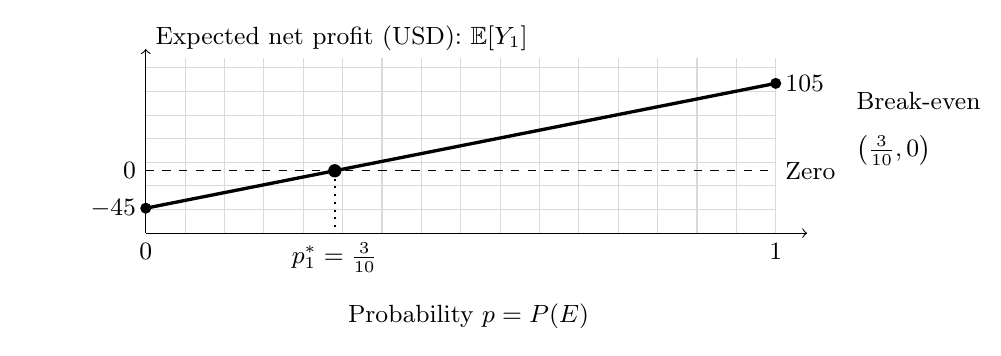
\begin{tikzpicture}[x=1cm,y=.6cm]
\path[use as bounding box] (0,-1) rectangle (12,5.35);
\draw[black!15,step=.5] (1.5,1) grid (9.5,4.7);
\draw[->] (1.5,1)--(9.9,1);
\draw[->] (1.5,1)--(1.5,4.9);
\node[anchor=west,font=\small,text=ExpectedInk] at (1.5,5.12) {Expected net profit (USD): $\EV{1}$};
\node[font=\small,text=ProbabilityInk] at (5.6,-.75) {Probability $\S{p}=P(\A{E})$};
\node[below,font=\small] at (1.5,1) {$0$};
\node[below,font=\small] at (9.5,1) {$1$};
\visible<2->{
\fill[ExpectedInk] (1.500,1.529) circle (2pt);
\fill[ExpectedInk] (9.500,4.171) circle (2pt);
\node[left,font=\small] at (1.500,1.529) {$\V{-45}$};
\node[right,font=\small] at (9.500,4.171) {$\V{105}$};
}
\visible<3->{\draw[ExpectedInk,very thick] (1.500,1.529)--(9.500,4.171);}
\visible<4->{
\draw[black,dashed] (1.5,2.321)--(9.5,2.321);
\node[left,font=\small] at (1.5,2.321) {$\V{0}$};
\node[right,font=\small] at (9.5,2.321) {Zero};
}
\visible<5->{
\draw[ProbabilityInk,thick,dotted] (3.900,2.321)--(3.900,1);
\fill[black] (3.900,2.321) circle (2.4pt);
\node[below,font=\small] at (3.900,1) {$\S{p_1^*}=\S{\frac3{10}}$};
\node[anchor=west,font=\small] at (10.4,3.8) {Break-even};
\node[anchor=west,font=\small] at (10.4,2.75) {$\bigl(\S{\frac3{10}},\V{0}\bigr)$};
}
\end{tikzpicture}

\end{frame}
% Frame 34: classroom 427--432 endpoint/root checks and sign interpretations
\SetTaskSubtask{2}{3}
\begin{frame}[t]{Food stand: connect graph, algebra and meaning}
\TaskBody

\Ask{Do the graph's endpoints and root agree with the formula?}
\visible<2->{\[\begin{aligned}
\EV{1}(0)&=-45+150(0)=\V{-45},\\[4pt]
\EV{1}(1)&=-45+150(1)=\V{105}\quad\text{USD}.
\end{aligned}\]}\par

\visible<3->{Root check: $\displaystyle -45+150(\frac3{10})=\V{0}$.
The endpoint expectations equal the given state payoffs.}\par

\medskip
\visible<4->{Above the zero line, $p\in\S{(\frac3{10},1]}$: \V{expected net gain}.
Below it, $p\in\S{[0,\frac3{10})}$: \V{expected net loss}.}\par


\end{frame}
% Frame 35: classroom 420--426 graphs; practice BreakEvenGraph semantic strokes; fixed bounds across overlays
\SetTaskSubtask{2}{3}
\begin{frame}[t]{Indoor games: expected-value graph}
\TaskBody

\Ask{How do the state payoffs and the zero threshold determine this graph?}
\centering
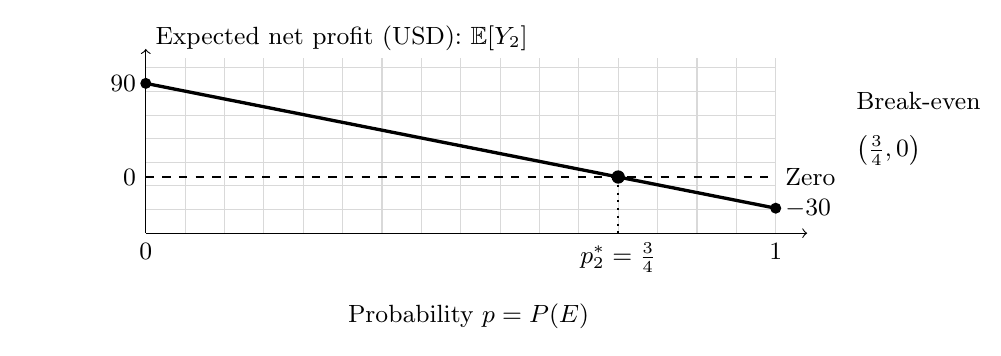
\begin{tikzpicture}[x=1cm,y=.6cm]
\path[use as bounding box] (0,-1) rectangle (12,5.35);
\draw[black!15,step=.5] (1.5,1) grid (9.5,4.7);
\draw[->] (1.5,1)--(9.9,1);
\draw[->] (1.5,1)--(1.5,4.9);
\node[anchor=west,font=\small,text=ExpectedInk] at (1.5,5.12) {Expected net profit (USD): $\EV{2}$};
\node[font=\small,text=ProbabilityInk] at (5.6,-.75) {Probability $\S{p}=P(\A{E})$};
\node[below,font=\small] at (1.5,1) {$0$};
\node[below,font=\small] at (9.5,1) {$1$};
\visible<2->{
\fill[ExpectedInk] (1.500,4.171) circle (2pt);
\fill[ExpectedInk] (9.500,1.529) circle (2pt);
\node[left,font=\small] at (1.500,4.171) {$\V{90}$};
\node[right,font=\small] at (9.500,1.529) {$\V{-30}$};
}
\visible<3->{\draw[ExpectedInk,very thick] (1.500,4.171)--(9.500,1.529);}
\visible<4->{
\draw[black,dashed] (1.5,2.189)--(9.5,2.189);
\node[left,font=\small] at (1.5,2.189) {$\V{0}$};
\node[right,font=\small] at (9.5,2.189) {Zero};
}
\visible<5->{
\draw[ProbabilityInk,thick,dotted] (7.500,2.189)--(7.500,1);
\fill[black] (7.500,2.189) circle (2.4pt);
\node[below,font=\small] at (7.500,1) {$\S{p_2^*}=\S{\frac34}$};
\node[anchor=west,font=\small] at (10.4,3.8) {Break-even};
\node[anchor=west,font=\small] at (10.4,2.75) {$\bigl(\S{\frac34},\V{0}\bigr)$};
}
\end{tikzpicture}

\end{frame}
% Frame 36: classroom 427--432 endpoint/root checks and sign interpretations
\SetTaskSubtask{2}{3}
\begin{frame}[t]{Indoor games: check graph and formula}
\TaskBody

\Ask{Do the graph's endpoints and root agree with the formula?}
\visible<2->{\[\begin{aligned}
\EV{2}(0)&=90-120(0)=\V{90},\\[4pt]
\EV{2}(1)&=90-120(1)=\V{-30}\quad\text{USD}.
\end{aligned}\]}\par

\visible<3->{Root check: $\displaystyle 90-120(\frac34)=\V{0}$.
The endpoint expectations equal the given state payoffs.}\par

\medskip
\visible<4->{Above the zero line, $p\in\S{[0,\frac34)}$: \V{expected net gain}.
Below it, $p\in\S{(\frac34,1]}$: \V{expected net loss}.}\par


\end{frame}
% Frame 37: classroom 427--432 and context 229; loss probabilities 325--345
\SetTaskSubtask{2}{3}
\begin{frame}[t]{Expectation describes an average, not a guarantee}
\TaskBody

\Ask{Does positive expectation guarantee profit on one weekend? Does break-even mean every payoff is zero?}
\visible<2->{No. At $p=3/8$, both expectations are positive, but the food stand still loses
\M{USD 45} with probability \Q{$5/8$}; games still lose \M{USD 30} with probability \S{$3/8$}.}\par

\medskip
\visible<3->{At its own break-even probability, each alternative has \V{zero long-run average}
net profit, although every realized payoff is nonzero:
\M{$-45$ or $105$} for food; \M{$-30$ or $90$} for games (USD).}\par

\medskip
\visible<4->{Both alternatives depend on the same concert outcome. Only one is chosen;
each threshold describes that alternative's individual expectation.}\par


\end{frame}

\section{Synthesis}
% Frame 38: synthesis of selected worked example 1, Tasks 1--2 only
\SetTaskSubtask{0}{0}
\begin{frame}[t]{From one event to an individual threshold}

\A{Binary event} $E$: concert goes ahead
$\longrightarrow$ \I{indicator} $X\in\{0,1\}$.
\medskip
\T{State-to-money rule} $f_i$ gives $\M{Y_i}=f_i(X)$ in USD.
\medskip
\Prob{Distribution and loss probability}: order the monetary payoffs;
attach the correct state masses and identify $\{Y_i<0\}$.
\medskip
\V{Expectation}: weight payoffs by their probabilities.
Hold payoffs fixed to obtain a line in $\S{p}$.
\medskip
\S{Individual break-even threshold}: solve $\mathbb E[Y_i]=0$;
interpret its positive and negative intervals as average net gains and losses.

\end{frame}

\section{Highlight recap}
% Frame 39: retrieval/consolidation: identical opening legend rows 1--4
\begin{frame}[t]{Highlight recap (1/3)}
\LegendOne
\end{frame}
% Frame 40: retrieval/consolidation: identical opening legend rows 5--8
\begin{frame}[t]{Highlight recap (2/3)}
\LegendTwo
\end{frame}
% Frame 41: retrieval/consolidation: identical opening legend rows 9--12
\begin{frame}[t]{Highlight recap (3/3)}
\LegendThree
\end{frame}
\end{document}



